Строится новый пиратский парусник. У парусника есть $N$ мачт, которые разделены на единичные
отрезки, при этом высота мачты равна количеству отрезков. На каждой мачте размещено некоторое
количество парусов, каждый из которых занимает один отрезок. Паруса на мачте могут быть размещены
произвольным образом по отрезкам, но в каждом отрезке может размещаться только один парус.

Разные расположения парусов обеспечивают различную тягу, когда на них дует ветер. Парус,
находящийся перед другими парусами на той же высоте, получает меньше ветра и дает меньше тяги. Для
каждого паруса определим показатель его неэффективности как суммарное количество парусов,
расположенных за этим парусом на той же высоте. Обратите внимание, что <<перед>> и <<за>> определяется
относительно положения корабля: на рисунке <<перед>> обозначает слева, <<за>>~--- справа.
Общий показатель неэффективности размещения парусов~--- это сумма показателей
неэффективности каждого из парусов. 


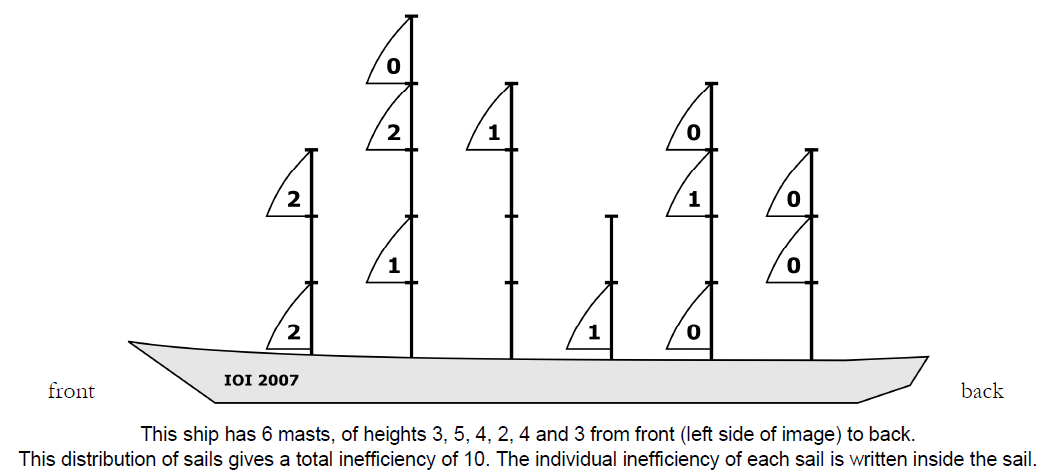
\includegraphics[scale=0.6]{sails.png}


Напишите программу, которая по заданной высоте и количеству парусов на каждой из $N$ мачт
определяет наименьший возможный общий показатель неэффективности. 